%%%%%%%%%%%%%%%%%%%%%%%%%%%%%%%%%%%%%%%%%
% Jacobs Landscape Poster
% LaTeX Template
% Version 1.0 (29/03/13)
%
% Created by:
% Computational Physics and Biophysics Group, Jacobs University
% https://teamwork.jacobs-university.de:8443/confluence/display/CoPandBiG/LaTeX+Poster
% 
% Further modified by:
% Nathaniel Johnston (nathaniel@njohnston.ca)
%
% This template has been downloaded from:
% http://www.LaTeXTemplates.com
%
% License:
% CC BY-NC-SA 3.0 (http://creativecommons.org/licenses/by-nc-sa/3.0/)
%
%%%%%%%%%%%%%%%%%%%%%%%%%%%%%%%%%%%%%%%%%

%----------------------------------------------------------------------------------------
%	PACKAGES AND OTHER DOCUMENT CONFIGURATIONS
%----------------------------------------------------------------------------------------

\documentclass[final, 13pt]{beamer}
\usepackage[utf8]{inputenc}
\usepackage[size=custom, width=44, height=36, scale=1.1]{beamerposter} 
%\usepackage[scale=1]{beamerposter} % Use the beamerposter package
                                % for laying out the poste
%\usepackage{caption}
%\captionsetup{format=plain, font=small, labelfont=bf}
%\usepackage[thinlines]{easytable}
\usetheme{confposter} % Use the confposter theme supplied with this template

\setbeamercolor{block title}{fg=ncsured,bg=white} % Colors of the block titles
\setbeamercolor{block body}{fg=black,bg=white} % Colors of the body of blocks
\setbeamercolor{block alerted title}{fg=white,bg=gray!70} % Colors of the highlighted block titles
\setbeamercolor{block alerted body}{fg=black,bg=gray!10} % Colors of the body of highlighted blocks
% Many more colors are available for use in beamerthemeconfposter.sty

%-----------------------------------------------------------
% Define the column widths and overall poster size
% To set effective sepwid, onecolwid and twocolwid values, first choose how many columns you want and how much separation you want between columns
% In this template, the separation width chosen is 0.024 of the paper width and a 4-column layout
% onecolwid should therefore be (1-(# of columns+1)*sepwid)/# of columns e.g. (1-(4+1)*0.024)/4 = 0.22
% Set twocolwid to be (2*onecolwid)+sepwid = 0.464
% Set threecolwid to be (3*onecolwid)+2*sepwid = 0.708

%The poster presentation space available is 3ft wide x 4ft high, or 36in w x 48 in h (0.92m wide  x 1.22m high). Dimensions are for a vertical poster. It is important to note that there is an approximately 1 inch metal rim on the border, which reduces the poster board VISIBLE space to 2 feet 10 inches wide by 3 feet 10 inches high. (1.17 meters x .86 meters).  

\newlength{\sepwid}
\newlength{\onecolwid}
\newlength{\twocolwid}
\newlength{\threecolwid}
\setlength{\paperwidth}{86cm} % A0 width: 46.8in
\setlength{\paperheight}{120cm} % A0 height: 33.1in
\setlength{\sepwid}{0.024\paperwidth} % Separation width (white space) between columns
\setlength{\onecolwid}{0.3\paperwidth} % Width of one column
\setlength{\twocolwid}{0.464\paperwidth} % Width of two columns
\setlength{\threecolwid}{0.708\paperwidth} % Width of three columns
\setlength{\topmargin}{-0.5in} % Reduce the top margin size
%-----------------------------------------------------------

\usepackage{graphicx}  % Required for including images

\usepackage{booktabs} % Top and bottom rules for tables

%----------------------------------------------------------------------------------------
%	TITLE SECTION 
%----------------------------------------------------------------------------------------



\title{ \hspace{-6.8cm} Characterization of the hexaploid sweetpotato inheritance using ultra-dense multilocus genetic map.} % Poster title

\author{Marcelo Mollinari \textsuperscript{1, 2, $*$ },
               Bode Olukolu  \textsuperscript{3},
               Guilherme Pereira da Silva \textsuperscript{1, 2}, 
               Awais Khan \textsuperscript{4},
               Dorcus C. Gemenet   \textsuperscript{5},
               \\Craig Yencho \textsuperscript{2},
               Zhao-Bang Zeng \textsuperscript{1, 2}}

\institute{1 Bioinformatics Research Center, North Carolina
  State University; 2 Department of Horticultural Sciences, North Carolina
  State University; 3 Department of Entomology and Plant Pathology, University of Tennessee; 
 4 Plant Pathology and Plant-Microbe Biology Section, Cornell University; 5 International Potato Center, ILRI Campus, Nairobi, Kenya; \textsuperscript{*}mmollin@ncsu.edu
}

%----------------------------------------------------------------------------------------

\begin{document}
\vspace{-20cm}


\addtobeamertemplate{block end}{}{\vspace*{2ex}} % White space under blocks
\addtobeamertemplate{block alerted end}{}{\vspace*{2ex}} % White space under highlighted (alert) blocks

\setlength{\belowcaptionskip}{2ex} % White space under figures
\setlength\belowdisplayshortskip{2ex} % White space under equations

\begin{frame}[t] % The whole poster is enclosed in one beamer frame

\begin{columns}[t] % The whole poster consists of three major columns,
  % the second of which is split into two columns twice - the [t]
  % option aligns each column's content to the top
\begin{column}{\sepwid}\end{column} % Empty spacer column

\begin{column}{\twocolwid} % The first column


%----------------------------------------------------------------------------------------
%	CONTEXT
%----------------------------------------------------------------------------------------
\begin{block}{Context}
The hexaploid sweetpotato (\textit{Ipomoea batatas} (L.) Lam., 2n = 6x = 90) is
an important staple food crop worldwide.  Despite its undeniable social and economic importance, genetic studies in sweetpotato significantly lag behind major diploid crops due to its complex hexapolyploid genome. To fully characterize the inheritance pattern in sweetpotato, we built an ultra-dense multilocus integrated genetic map of a full-sib population derived from a cross between the cultivars ‘Beauregard’ and ‘Tanzania’ (BT population) using our newly implemented software, MAPpoly~\textsuperscript{1}. Using the genotypic probabilities computed across all linkage groups, we  inferred the complete hexaploid haplotypes for all individuals in the offspring and evaluated the levels of preferential pairing and multivalent formation. 
\end{block}

\vspace{1.450cm}
%----------------------------------------------------------------------------------------
%	MAPING POPULATION AND GENOTYPE CALLING
%----------------------------------------------------------------------------------------
\begin{block}{Mapping population and genotype calling}
    \begin{itemize}
      \item Biparental cross: ‘Beauregard’ $\times$ ‘Tanzania’, 315
        full-sib progeny.%\vspace{.75cm}
    \item Genotyping: modified GBS protocol optimized for polyploids
      (GBSpoly)\textsuperscript{2} using the genome of two diploid sweetpotatoes, 
      \textit{I. trifida} and \textit{I. triloba}\textsuperscript{3}, as reference. %\vspace{.75cm}
    \item SNP calling using SuperMASSA\textsuperscript{4}. %\vspace{.75cm}
      %\begin{center}
      %\includegraphics[width=.7\textwidth]{figures/super.png}
      %\end{center}
      \item After filtering, a total of 38,701 high
        confidence SNPs were used to build the map. %\vspace{.75cm}
         \item The probability distribution of the genotypes was incorporated in a HMM to model the genotyping errors\textsuperscript{5}.
    \end{itemize}
    
    \begin{figure}[htp]\label{fig:info}
      \centering
      \includegraphics[width=0.7\textwidth]{figures/Tf_S1_30010438.jpg}
      \caption{\hspace{.01cm} Example of genotype call of SNP \textit{Tf\_S1\_30010438}. (A) Scatter plot of the read counts for the two allelic variants A and G. (B) Inferred probability distribution of genotypes for each individual in the offspring. Loci where the highest posterior probability was smaller than 0.8 were assigned as missing data (gray dots).}
    \end{figure}
  \end{block}
%----------------------------------------------------------------------------------------
%	TWO-POINT ANALYSIS AND SNP ORDERING
%----------------------------------------------------------------------------------------
%  \begin{block}{Two-point analysis and SNP ordering}
%  \begin{itemize}
%  \item Two-point recombination fraction estimates were
%    obtained by reducing the complexity of a general HMM using a
%    computational approach \cite{Mollinari2019}
%   \end{itemize}
%  \begin{figure}[htp]\label{fig:haplo}
%    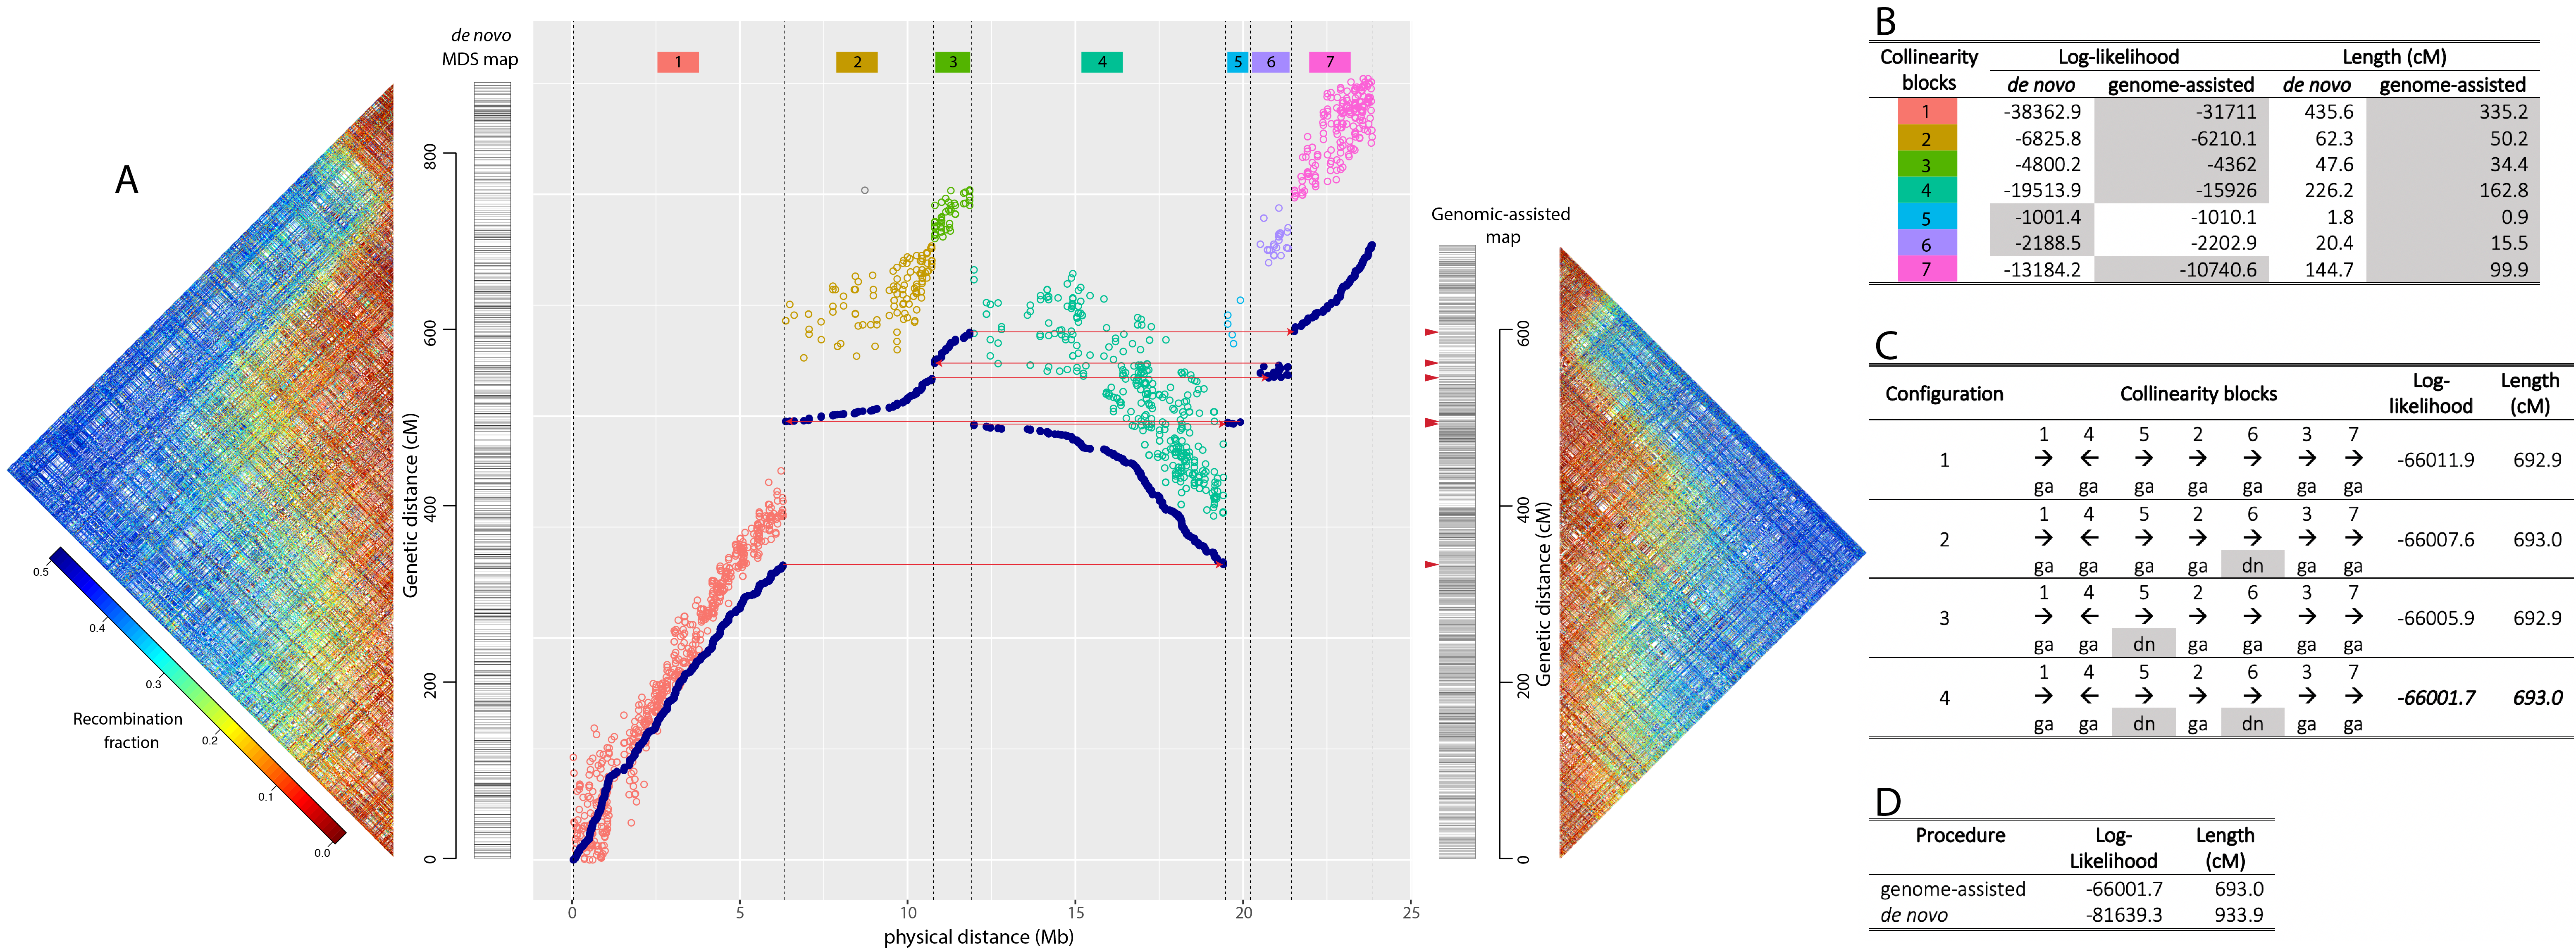
\includegraphics[width=.5\textwidth]{figures/geno_assist_ch7.png}
%    \caption{\hspace{.01cm} Schematic overview of the map order improvement using \textit{I. trifida} reference genome in linkage group  7. (A) Scatter plot of the physical distance in \textit{I. trifida} reference genome (horizontal axis) versus the genetic distance in the de novo genetic map (colored dots) and the genome-assisted genetic map (dark blue dots). (B) Multilocus log-likelihood and the final length of each collinearity block. (C) Complete map models concatenating all seven collinearity blocks. (D) Final comparison of de novo and genome-assisted map, indicating a clear superiority of the latter.}
%  \end{figure}
%\end{block}

%----------------------------------------------------------------------------------------
%	SWEETPOTATO GENETIC MAP
%----------------------------------------------------------------------------------------
\begin{block}{Sweetpotato phased genetic map}
  \begin{itemize}
  \item 15 linkage groups consistent with the chromosomes of the diploid reference genomes
  \item Multidimensional Scaling Algorithm (MDS)\textsuperscript{6} was used to order
    SNPs \textit{I. trifida} reference genome was used to propose alternative SNP orders within collinearity blocks and evaluated 
  the likelihood of the resulting maps.
  \item Multilocus fully phased map containing 30,684 SNPs (60.7\% simplex and double-simplex, and 39.3\% multiplex markers) spanning 2,708.4 cM.
  \item 81.9\% of all map positions in ‘Beauregard’ and 77.2\% in ‘Tanzania’ had a GIC > 80\%
  %\item Thirty-nine blocks were aligned to 326.5 Mb of \textit{I. trifida} genome, covering 96.5\% of the \textit{I. batatas} map (2,614.8 cM), with an average density of one SNP/14.2 kb; 107 blocks were aligned to 258.8 Mb of \textit{I. triloba} genome, covering 83.1\% of the map (2,251.8 cM), with an average density of one SNP/13.4 kb. The averaged genetic to physical map ratios for these regions were of ~124.8 kb per cM for \textit{I. trifida} and ~114.9 kb per cM for \textit{I. triloba}.
  \end{itemize}
  \begin{figure}[htp]\label{fig:haplo}
    \includegraphics[width=.9\textwidth]{figures/final_map.jpg}
    \caption{\hspace{.01cm} Sweetpotato genetic map\textsuperscript{7}. Blue lines connecting the map and reference genomes indicate SNPs shared between \textit{I. trifida} and \textit{I. triloba} reference genomes and red lines indicate private SNPs. Above each map, we present a graphical representation of the parental linkage phase configuration of the homology groups for parents ‘Beauregard’ and ‘Tanzania’. The Genotypic Information Content (GIC), is presented below each homology group.}
  \end{figure} 
  \end{block}
  \end{column} % End of the first column

\begin{column}{\sepwid}\end{column} % Empty spacer column

\begin{column}{\twocolwid} % The third column
%----------------------------------------------------------------------------------------
%	HAPLOTYPE RECONSTRUCTION AND MULTIVALENT FORMATION
%----------------------------------------------------------------------------------------
\begin{block}{Haplotype reconstruction and multivalent formation}
    
\begin{itemize}
\item Most of the meiotic configurations (73.3\%) were resolved in bivalents, although a small portion of multivalent signatures (15.7\%), and inconclusive configurations (11.0\%) were also observed.
\end{itemize}    
    
    
 \begin{figure}[htp]
      \centering
      \includegraphics[width=0.8\textwidth]{figures/haplotype_reconstruction.png}
      \caption{\hspace{.01cm} Example of haplotype reconstruction and distribution of meiotic configurations for individual BT05.320, linkage group 1. (A) and (B) Probability profiles for 12 homologs indicating the segments inherited from parents ‘Beauregard’ and ‘Tanzania’, respectively.  The arrows indicate recombination points; (C) Recombination signature table; (D) Possible meiotic configuration that originated gametes for individual BT05.320 in ‘Beauregard’ and ‘Tanzania’ and resulting gamete. E) Representation of the meiotic results as a graph where nodes represent the homologs and the edges represent recombination events.} 
    \end{figure}  
\end{block}

%----------------------------------------------------------------------------------------
%	PREFERENTIAL PAIRING
%----------------------------------------------------------------------------------------

\begin{block}{Preferential Pairing}
    \begin{itemize}
    \item Except for low levels of preferential pairing in linkage group 2, we observed a hexasomic inheritance mechanism in all linkage groups.    

    \end{itemize}
    
 \begin{figure}[htp]
      \centering
      \includegraphics[width=0.9\textwidth]{figures/homolog_preferential_pairing_profiles2.png}
      \caption{\hspace{.01cm}Probability profiles for 15 homolog pairs in parents ‘Beauregard’ and ‘Tanzania’ across 15 linkage groups. The dashed lines in the probability profiles indicate the pairing probability expected under random pairing ($\frac{3}{15} = 0.2$).
 The lower panels indicate $-\log_{10}P$ of a $\chi^2$ independence test for all possible homolog pairs. Dashed lines indicate $P < 10^{-4}$. Homologs $i$ and $j$ presented a low, but significant preferential pairing in linkage group 2.} 
    \end{figure}  
\end{block}


%----------------------------------------------------------------------------------------
%	CONCLUSION
%----------------------------------------------------------------------------------------
\vspace{-.750cm}
\begin{block}{Conclusion}

\begin{itemize}
\item Although compute-intensive, the construction of multipoint genetic maps in complex polyploids has several advantages, including error modeling, computation of preferential pairing profiles, and construction of haplotypes in the offspring.
\item The resulting sweetpotato genetic map revealed 96.5\% collinearity between the hexaploid  \textit{I. batatas} and its diploid relative \textit{I. trifida}. 
\item We showed that sweetpotato inheritance is vastly autopolyploid-like and random chromosome pairing enables recombination between all homologous across generations.
\item We speculate that the hexasomic-bivalent inheritance promotes stability to the allelic transmission in sweetpotato.
\end{itemize}
 Related talk in this conference: Sweetpotato Genomics Workshop - Characterization of Sweetpotato Inheritance Using Ultradense Multilocus Genetic Map (Royal Palm Salon 5-6, Wednesday, Jan 15, 1:55 PM)
\end{block}

%----------------------------------------------------------------------------------------
%	REFERENCES
%----------------------------------------------------------------------------------------

\begin{block}{References}
\begin{small}
1. \url{https://github.com/mmollina/mappoly} \\
2. Wald \textit{et al.} 2018. doi: 10.3389/fpls.2018.01166 \\
3. Wu \textit{et al.} 2018. doi: 10.1038/s41467-018-06983-8\\
4. Serang \textit{et al.} 2012. doi: 10.1371/journal.pone.0030906\\
5. Mollinari and Garcia 2019. doi: 10.1534/g3.119.400378 \\
6. Preedy and Hackett 2016. doi: 10.1007/s00122-016-2761-8\\
7. Mollinari \textit{et al.} 2020. doi: 10.1534/g3.119.400620\\
\end{small}

\end{block}


%----------------------------------------------------------------------------------------
%	CONTACT INFORMATION
%----------------------------------------------------------------------------------------

\setbeamercolor{block alerted title}{fg=black,bg=norange} % Change the alert block title colors
\setbeamercolor{block alerted body}{fg=black,bg=white} % Change the alert block body colors

%\vspace{-4.0cm}
%\begin{flushright}
%\scriptsize Financial Support\\
%\includegraphics[width=.45\linewidth]{fapesp.png} 
%\end{flushright}

%----------------------------------------------------------------------------------------

\end{column} % End of the fourth column

\end{columns} % End of all the columns in the poster

\end{frame} % End of the enclosing frame

\end{document}
